% Figura de arquitectura: GPT-2 con capas MoE alternas.
% Colores según la convención de Vaswani et al. (2017): embedding rosa,
% atención naranja, Add & Norm amarillo, FFN azul, lineal lavanda.
% La capa MoE va en verde para distinguirla de la FFN densa.
% Compilar con: pdflatex moe_block.tex  ->  moe_block.pdf
\documentclass[border=3pt]{standalone}
\usepackage[T1]{fontenc}
\usepackage{mathptmx}
\usepackage{tikz}
\usetikzlibrary{calc,arrows.meta,decorations.pathreplacing}

% ---------- Paleta ----------
\definecolor{emb}{HTML}{F29B9B}
\definecolor{att}{HTML}{F7B267}
\definecolor{ln}{HTML}{EFE07A}
\definecolor{ffn}{HTML}{8EC5EA}
\definecolor{moe}{HTML}{6CC08B}
\definecolor{lin}{HTML}{B9B3E6}
\definecolor{router}{HTML}{CDEBD7}
\definecolor{sel}{HTML}{2B6CB0}
\definecolor{idle}{HTML}{E6E6E6}
\definecolor{frame}{HTML}{5A6B7D}

% \slab{x}{y}{ancho}{alto}{color}: prisma 3D centrado en (x,y)
\newcommand{\slab}[5]{%
  \fill[#5!70!black] ({#1+#3/2},{#2-#4/2}) -- ++(0.12,0.12) -- ++(0,#4) -- ++(-0.12,-0.12) -- cycle;
  \fill[#5!55!white] ({#1-#3/2},{#2+#4/2}) -- ++(0.12,0.12) -- ++(#3,0) -- ++(-0.12,-0.12) -- cycle;
  \fill[#5] ({#1-#3/2},{#2-#4/2}) rectangle ({#1+#3/2},{#2+#4/2});
  \draw[#5!50!black, line width=0.3pt] ({#1-#3/2},{#2-#4/2}) rectangle ({#1+#3/2},{#2+#4/2})
    ({#1+#3/2},{#2+#4/2}) -- ++(0.12,0.12) -- ++(0,-#4) -- ++(-0.12,-0.12)
    ({#1-#3/2},{#2+#4/2}) -- ++(0.12,0.12) -- ++(#3,0);
}

\tikzset{
  >={Stealth[length=4pt,width=3pt]},
  flow/.style={->, line width=0.6pt},
  res/.style={->, line width=0.6pt, rounded corners=3pt},
  lab/.style={font=\scriptsize, align=center, inner sep=1pt},
  sum/.style={circle, draw, line width=0.6pt, fill=white, inner sep=0pt, minimum size=11pt},
  panel/.style={draw=frame, dashed, line width=0.8pt, rounded corners=6pt},
  ptitle/.style={font=\footnotesize\bfseries, text=frame!80!black},
  zoom/.style={gray!60, dashed, line width=0.4pt},
  rbox/.style={draw=moe!50!black, fill=router, rounded corners=1.5pt, lab, minimum height=0.45cm, minimum width=1.1cm},
  pick/.style={->, sel, line width=1pt},
}

\begin{document}
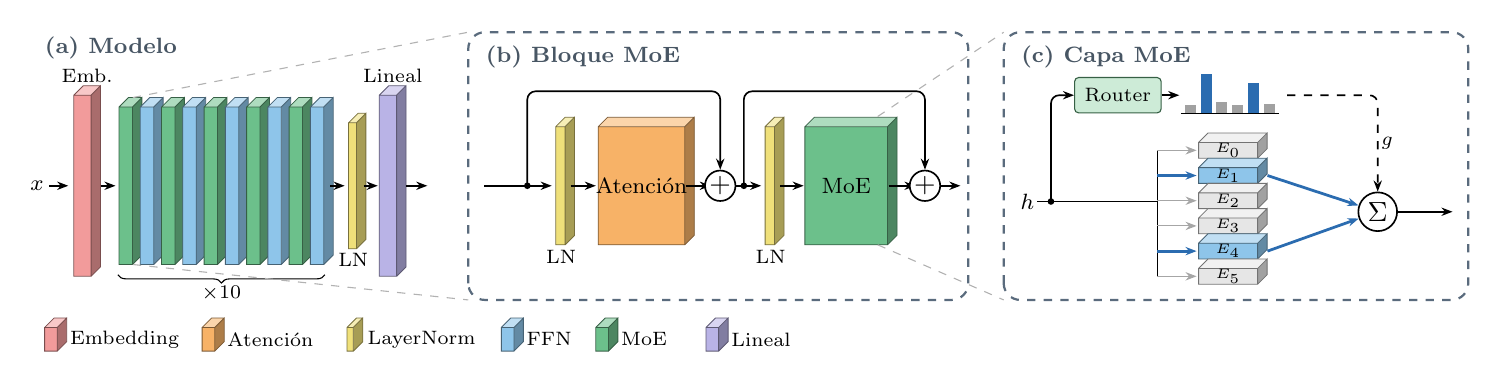
\begin{tikzpicture}

% ---------- (a) Modelo ----------
\node[ptitle, anchor=west] at (0,1.75) {(a) Modelo};
\node[lab, anchor=east] at (0.15,0) {\footnotesize $x$};
\draw[flow] (0.18,0) -- (0.42,0);
\slab{0.6}{0}{0.22}{2.3}{emb}
\node[lab, above] at (0.66,1.27) {Emb.};
\draw[flow] (0.83,0) -- (1.02,0);
\foreach \i in {0,...,9} {
  \pgfmathsetmacro{\x}{1.15+\i*0.27}
  \pgfmathparse{mod(\i,2)==0 ? "moe" : "ffn"}
  \edef\c{\pgfmathresult}
  \slab{\x}{0}{0.17}{2.0}{\c}
}
\draw[decorate, decoration={brace, mirror, amplitude=3pt}, line width=0.4pt]
  (1.05,-1.13) -- (3.68,-1.13) node[midway, below=3pt, lab] {$\times10$};
\draw[flow] (3.75,0) -- (3.93,0);
\slab{4.03}{0}{0.1}{1.6}{ln}
\node[lab, below] at (4.04,-0.82) {LN};
\draw[flow] (4.17,0) -- (4.35,0);
\slab{4.48}{0}{0.22}{2.3}{lin}
\node[lab, above] at (4.54,1.27) {Lineal};
\draw[flow] (4.71,0) -- (4.98,0);
\draw[zoom] (1.24,1.12) -- (5.5,1.95);
\draw[zoom] (1.24,-1.0) -- (5.5,-1.45);

\begin{scope}[xshift=0.75cm]
% ---------- (b) Bloque MoE ----------
\draw[panel] (4.75,-1.45) rectangle (11.1,1.95);
\node[ptitle, anchor=north west] at (4.85,1.9) {(b) Bloque MoE};

\coordinate (s1) at (5.5,0);
\draw[line width=0.6pt] (4.95,0) -- (s1);
\fill (s1) circle (1.2pt);
\draw[flow] (s1) -- (5.81,0);
\slab{5.92}{0}{0.12}{1.5}{ln}
\node[lab, below] at (5.93,-0.78) {LN};
\draw[flow] (6.05,0) -- (6.37,0);
\slab{6.95}{0}{1.1}{1.5}{att}
\node[lab, font=\footnotesize] at (6.95,0) {Atención};
\draw[flow] (7.51,0) -- (7.83,0);
\node[sum] (p1) at (7.95,0) {$+$};
\draw[res] (s1) |- (6.45,1.2) -| (p1.north);

\coordinate (s2) at (8.25,0);
\draw[line width=0.6pt] (p1.east) -- (s2);
\fill (s2) circle (1.2pt);
\draw[flow] (s2) -- (8.47,0);
\slab{8.58}{0}{0.12}{1.5}{ln}
\node[lab, below] at (8.59,-0.78) {LN};
\draw[flow] (8.71,0) -- (9.01,0);
\slab{9.55}{0}{1.05}{1.5}{moe}
\node[lab, font=\footnotesize] at (9.55,0) {MoE};
\draw[flow] (10.09,0) -- (10.43,0);
\node[sum] (p2) at (10.55,0) {$+$};
\draw[res] (s2) |- (8.95,1.2) -| (p2.north);
\draw[flow] (p2.east) -- (11.0,0);

% ---------- (c) Capa MoE ----------
\draw[panel] (11.55,-1.45) rectangle (17.45,1.95);
\node[ptitle, anchor=north west] at (11.65,1.9) {(c) Capa MoE};
\draw[zoom] (9.95,0.88) -- (11.55,1.95);
\draw[zoom] (9.95,-0.75) -- (11.55,-1.45);

\node[lab, font=\footnotesize] (x) at (11.85,-0.2) {$h$};
\coordinate (bx) at (12.15,-0.2);
\draw[line width=0.6pt] (x.east) -- (bx);
\fill (bx) circle (1.2pt);
\node[rbox] (rt) at (13.0,1.15) {Router};
\draw[res] (bx) |- (rt.west);

% probabilidades del router (top-2 resaltado)
\foreach \i/\p in {0/0.10, 1/0.50, 2/0.14, 3/0.10, 4/0.38, 5/0.12} {
  \pgfmathsetmacro{\bx}{13.85+\i*0.2}
  \pgfmathparse{(\i==1 || \i==4) ? "sel" : "idle!70!black"}
  \edef\c{\pgfmathresult}
  \fill[\c] (\bx,0.92) rectangle ++(0.14,\p);
}
\draw[line width=0.4pt] (13.8,0.92) -- (15.04,0.92);
\draw[flow] (rt.east) -- (13.78,1.15);

% expertos (FFN): activos en azul, inactivos en gris
\foreach \i/\st in {0/idle, 1/ffn, 2/idle, 3/idle, 4/ffn, 5/idle} {
  \pgfmathsetmacro{\y}{0.45-\i*0.32}
  \slab{14.4}{\y}{0.75}{0.2}{\st}
  \node[lab, font=\tiny] at (14.4,\y) {$E_{\i}$};
}
\draw[line width=0.6pt] (bx) -- (13.5,-0.2);
\draw[line width=0.5pt] (13.5,0.45) -- (13.5,-1.15);
\foreach \i in {0,2,3,5} \draw[->, black!35, line width=0.4pt] (13.5,0.45-\i*0.32) -- (14.0,0.45-\i*0.32);
\foreach \i in {1,4} \draw[pick] (13.5,0.45-\i*0.32) -- (14.0,0.45-\i*0.32);

\node[sum, minimum size=14pt] (sg) at (16.3,-0.33) {$\Sigma$};
\draw[pick] (14.9,0.13) -- (sg);
\draw[pick] (14.9,-0.83) -- (sg);
\draw[res, dashed] (15.15,1.15) -| node[lab, pos=0.75, right] {$g$} (sg.north);
\draw[flow] (sg.east) -- (17.25,-0.33);

\end{scope}

% ---------- Leyenda ----------
\begin{scope}[shift={(0.2,-1.95)}, every node/.style={lab, anchor=west}]
  \slab{0}{0}{0.16}{0.3}{emb}      \node at (0.2,0)   {Embedding};
  \slab{2.0}{0}{0.16}{0.3}{att}    \node at (2.2,0)   {Atención};
  \slab{3.8}{0}{0.08}{0.3}{ln}     \node at (3.98,0)  {LayerNorm};
  \slab{5.8}{0}{0.16}{0.3}{ffn}    \node at (6.0,0)   {FFN};
  \slab{7.0}{0}{0.16}{0.3}{moe}    \node at (7.2,0)   {MoE};
  \slab{8.4}{0}{0.16}{0.3}{lin}   \node at (8.6,0)  {Lineal};
\end{scope}

\end{tikzpicture}
\end{document}
